% !TEX root =  ../main_manuscript.tex 
\section{Results}
The rate of upgrading at year five of follow-up was 35\% in PRIAS, and at most 50\% in the five validation GAP3 cohorts (Panel~B, Figure~\ref{fig:auc_beforecalib}). That is, many patients do not require any biopsy in the first five years of AS. 

In the fitted joint model, when patient age increased from 61 to 71 years (25-th to 75-th percentile), the adjusted hazard ratio of upgrading was 1.45~(95\%CI:~1.30--1.63). When fitted PSA value (log scale) increased from 2.36 to 3.07 (25-th to 75-th percentile), the adjusted hazard ratio was 0.99~(95\%CI:~0.89--1.11). When estimated instantaneous PSA (log scale) velocity increased from -0.09 to 0.31 (25-th to 75-th percentile), the adjusted hazard ratio was 2.47~(95\%CI:~1.93--2.99). Hence, instantaneous velocity of PSA was a stronger predictor of upgrading than PSA value. Detailed parameter estimates are in Supplementary~A.2.

The time-varying mean absolute prediction error, time-varying AUC, and calibration plot of our model in different cohorts are shown in Panel~B, Figure~8, Supplementary~B; Panel~A, Figure~\ref{fig:auc_beforecalib}; and Panel~B, Figure~\ref{fig:auc_beforecalib}, respectively. The AUC was moderate (0.55 to 0.75) in all cohorts. Mean absolute prediction error was large (0.3 to 0.45) in cohorts with rate of upgrading different from PRIAS, and moderate (0.1 to 0.3) otherwise. Our model required recalibration of baseline hazard of upgrading in all cohorts (Figure~6, Supplementary~B). Although, calibration was fine in Johns Hopkins cohort, whose rate of upgrading was similar to PRIAS (Panel~B, Figure~\ref{fig:auc_beforecalib}). The risk predictions from the recalibrated models were as good as risk predictions from joint models fitted separately to each cohort (Figure~7, Supplementary~B). Comprehensive validation results are in Supplementary~B.

\begin{figure}
\centerline{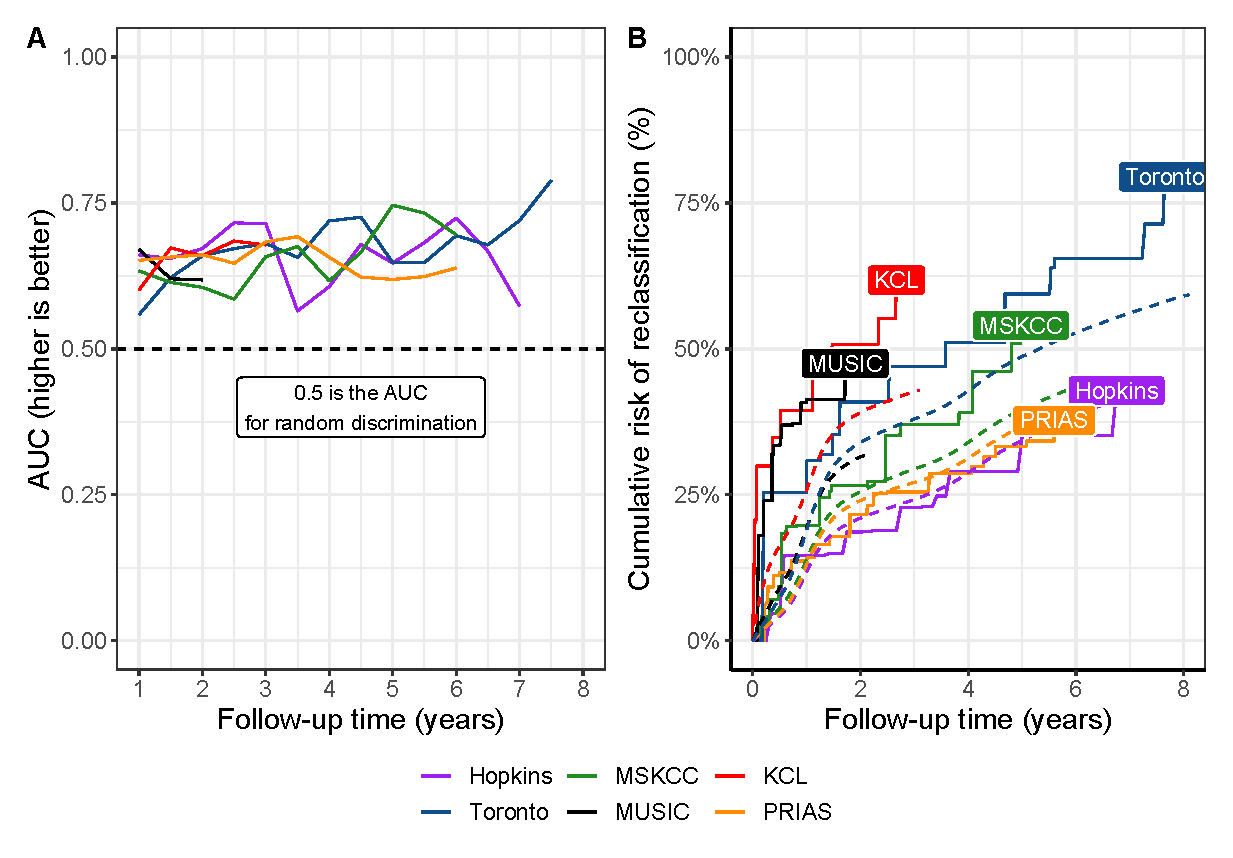
\includegraphics[width=\columnwidth]{images/auc_beforecalib.eps}}
\caption{\textbf{Model Validation Results}. \textbf{Panel~A}: time dependent area under the receiver operating characteristic curve or AUC (measure of discrimination). \textbf{Panel~B}: calibration-at-large~\citep{royston2013external,steyerberg2010assessing}, with solid lines depicting the non-parameteric estimate of the cumulative-risk of upgrading~\citep{turnbull1976empirical}, and dashed lines showing the average cumulative-risk of upgrading obtained using the joint model fitted to the PRIAS dataset. Full names of Cohorts are \textit{PRIAS}: Prostate Cancer International Active Surveillance, \textit{Toronto}: University of Toronto Active Surveillance, \textit{Hopkins}: Johns Hopkins Active Surveillance, \textit{MSKCC}: Memorial Sloan Kettering Cancer Center Active Surveillance, \textit{KCL}: King's College London Active Surveillance, \textit{MUSIC}: Michigan Urological Surgery Improvement Collaborative Active Surveillance.}
\label{fig:auc_beforecalib}
\end{figure}

\subsection{Personalized Biopsy Schedules}

The key component in personalized schedules is the cumulative-risk of upgrading. Given a patient's accumulated PSA measurements and biopsy results, our joint model predicted the cumulative-risk of upgrading at his current as well as future visit times (Panel~C, Figure~\ref{fig:jmExplanationPlot_113}). This cumulative-risk is updated with more patient data over follow-up (Figure~5, Supplementary~B).

In PRIAS, patient PSA was measured every six months. If during a PSA visit, a patient's predicted cumulative-risk of upgrading was more than a certain threshold (e.g., 10\%), we scheduled an immediate biopsy. We scheduled future biopsies too because our model predicts patient's cumulative-risk at his future follow-up visits as well. We achieved this by repeatedly applying the same risk threshold rule at each future follow-up visit (Supplementary~C). We maintained a minimum gap of one year between consecutive biopsies (PRIAS recommendation). Example personalized schedules based on 5\% and 10\% risk thresholds are shown in Panel~B, Figure~\ref{fig:demo_pat1}. Due to the currently limited follow-up period of PRIAS, we were able to schedule biopsies during the first six years of follow-up only (Table 12, Supplementary~C).

\begin{figure}[!htb]
\centerline{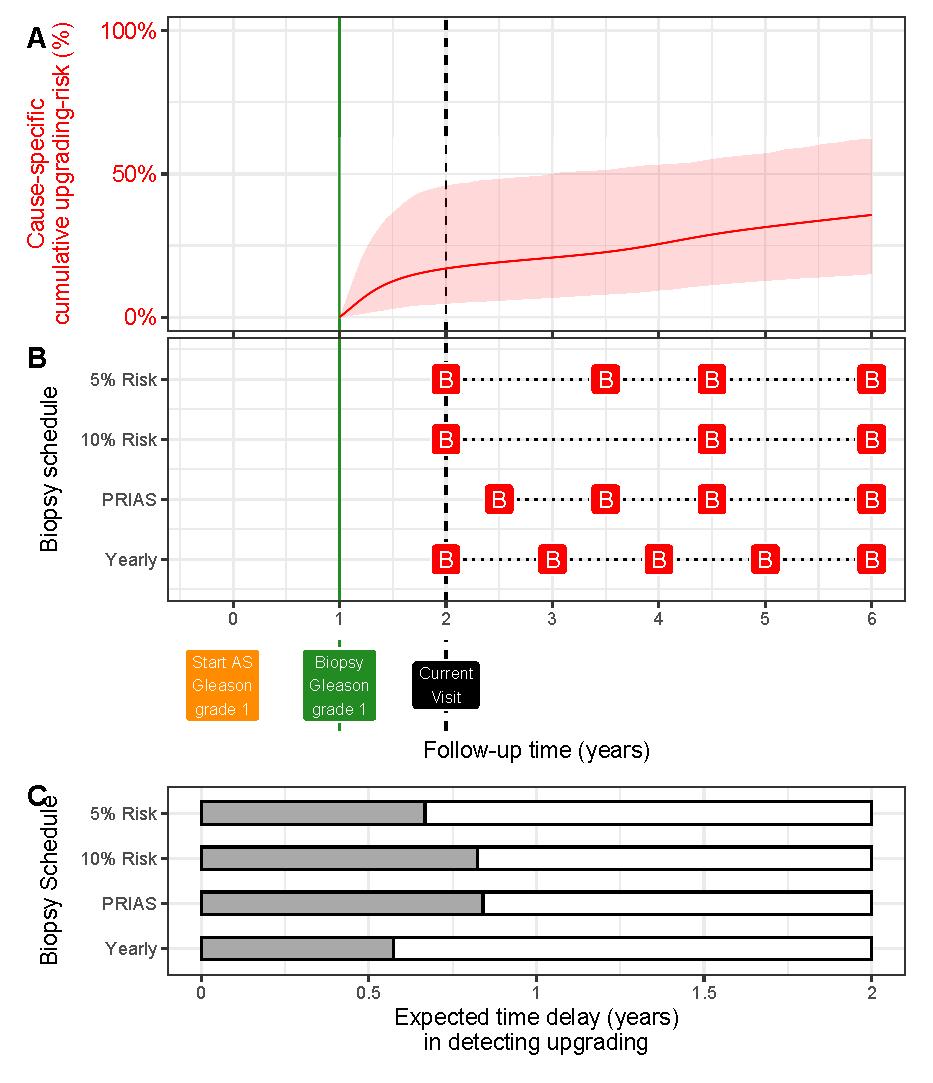
\includegraphics[width=\columnwidth]{images/demo_pat1.eps}}
\caption{\textbf{Illustration of personalized and fixed schedules of biopsies}. The PSA profile of this patient is shown in Figure~\ref{fig:jmExplanationPlot_113}. \textbf{Panel~A:} Predicted cumulative-risk of upgrading (95\% credible interval shaded). \textbf{Panel~B:} Personalized and fixed schedules of biopsies, with a red `B' indicating a scheduled biopsy. Green vertical line at year 1 denotes the time of latest negative biopsy. Black dashed line at year 3 denotes time of current visit. \textbf{Panel~C:}\ Expected time delay in detecting upgrading (months) for different schedules.}
\label{fig:demo_pat1}
\end{figure}

The choice of the risk threshold in the personalized schedule dictates the \textit{consequences} of following that schedule. \textit{Consequences} are the timing and the total number of biopsies, and the expected time delay in detecting upgrading. Our model estimated \textit{consequences} in a personalized manner (Panel~B,C in Figure~\ref{fig:demo_pat1}, and Figure~9--11 in Supplementary~C) given any schedule of biopsies. Thus, patients can compare personalized schedules based on different risk thresholds, with fixed schedules, before making a choice.

Various personalized and fixed biopsy schedules for a demonstration patient in Figure~\ref{fig:demo_pat1} show that a personalized schedule based on 10\% risk threshold leads to one less biopsy than other schedules. At the same time, the corresponding time delay in detection of upgrading is expected to be only one month more than other schedules. A compulsory biopsy was scheduled at year six (maximum biopsy scheduling time in PRIAS, Supplementary~C) in all schedules for a meaningful comparison between them. Additional demonstrations are in Figure~9--11, Supplementary~C.

\subsection{Web-Application}
We implemented our methodology in a web-application \url{https://emcbiostatistics.shinyapps.io/prias_biopsy_recommender/}. It utilizes the joint model fitted to the PRIAS dataset. Currently, the web-application supports PRIAS and the five external cohorts in which we validated our model. Patient data can be entered manually or can be uploaded in Microsoft Excel format. Predictions for risk of upgrading are shown for a currently limited, cohort-specific, follow-up period (Table 12, Supplementary~C). The web-application allows comparison of the \textit{consequences} of following these schedules: personalized schedules based on 5\%, 10\%, and 15\% risk threshold; annual biopsies; biennial biopsies; and PRIAS schedule.